% !TEX root = ../main.tex
% 本文件由 build-tex.sh 从 22-DSP指南-第22章中译.md 生成，改内容请改 md 后重新生成

\chapter{音频处理}\label{ch-22}

音频处理(audio
processing)涵盖许多不同的领域，它们都与把声音呈现给人类听众有关。其中有三个领域最为突出：(1)
高保真音乐重放，比如音频 CD；(2)
语音通信，也就是电话网络的另一种说法；(3)
合成语音，即由计算机生成和识别人的语音。这些应用的目标和难题各不相同，但它们由同一位裁判联系在一起：人耳。数字信号处理已经给这些以及音频处理的其他领域带来了革命性的变化。

\section{人的听觉}

人耳是一个极其复杂的器官。更麻烦的是，来自两只耳朵的信息还要在一个令人费解的神经网络------人脑------中合并。请记住，下面只是一个简短的概述；与人的听觉相关的微妙效应和尚未弄清的现象还有很多。

图 22-1 画出了构成人耳的主要结构和过程。外耳(outer
ear)由两部分组成：一是长在头侧、看得见的皮肤和软骨组成的耳廓，二是耳道(ear
canal)，一根直径约 0.5 cm、向头内延伸约 3 cm
的管子。这些结构把环境中的声音引向位于颅骨内部、受到安全保护的敏感的中耳和内耳器官。耳道末端绷着一层薄薄的组织，叫鼓膜(tympanic
membrane，ear drum)。声波打在鼓膜上，使它振动。中耳(middle
ear)是一组小骨头，把这种振动传到耳蜗(cochlea，即内耳)，在那里转换成神经冲动。耳蜗是一根充满液体的管子，直径约
2 mm，长约 3 cm。虽然图 22-1
把它画成直的，但耳蜗其实是盘卷起来的，看上去像个小蜗牛壳。事实上，cochlea
一词就来自希腊语的''蜗牛''。

\begin{figure}[htbp]
\centering
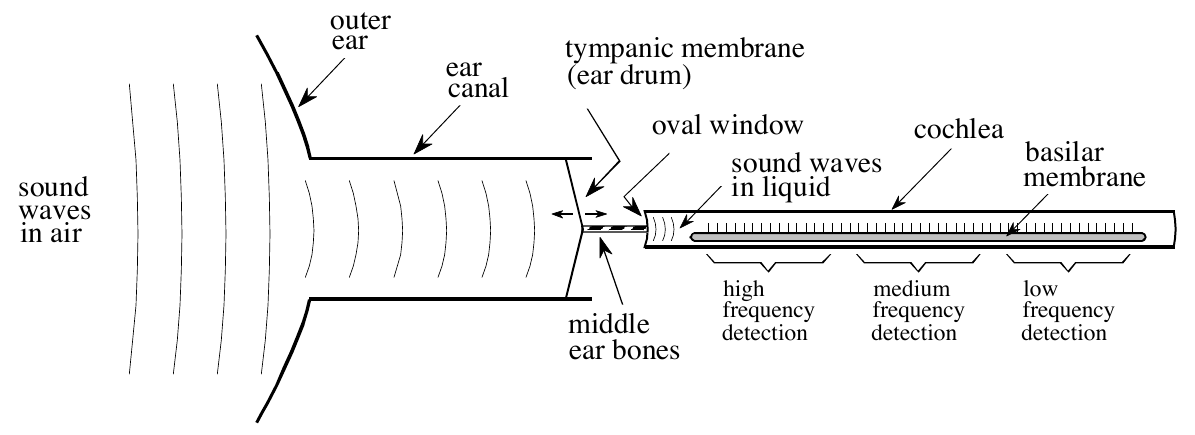
\includegraphics[width=0.996\linewidth,height=0.8\textheight,keepaspectratio]{assets/ch22/fig22-01.png}
\caption*{\textbf{图 22-1　人耳的功能示意图。}
外耳收集环境中的声波，把它们导向鼓膜。鼓膜是一层薄薄的组织，随空气中的波形同步振动。中耳的听小骨（锤骨、砧骨和镫骨）把这些振动传到卵圆窗------充满液体的耳蜗上的一层柔软的膜。耳蜗里有基底膜，它支撑着约
12,000
个构成耳蜗神经的神经细胞。由于基底膜各处的硬度不同，每个神经细胞只对很窄的一段音频频率有反应，这使耳朵成了一台频谱分析仪。
（sound waves in air = 空气中的声波，outer ear = 外耳，ear canal =
耳道，tympanic membrane (ear drum) = 鼓膜，middle ear bones =
听小骨，oval window = 卵圆窗，sound waves in liquid =
液体中的声波，cochlea = 耳蜗，basilar membrane = 基底膜，high / medium /
low frequency detection = 高 / 中 / 低频检测。原书图注把 responds 误写成
responses。）}
\end{figure}

声波试图从空气进入液体时，只有一小部分声音能穿过分界面，其余能量都被反射回去。这是因为空气的机械阻抗(mechanical
impedance)低（密度低、可压缩性高，所以声压低、质点速度高），而液体的机械阻抗高。用不那么专业的话说，在水里挥手比在空气里挥手费劲。机械阻抗的这种差异，使得大部分声音在空气/液体界面上被反射。

中耳是一个阻抗匹配网络，用来提高进入内耳液体的声能比例。比如鱼就没有鼓膜和中耳，因为它们不需要在空气中听声音。阻抗转换主要来自鼓膜（从空气接收声音）与卵圆窗(oval
window，把声音传入液体，见图 22-1)的面积差。鼓膜面积约 60
mm²，而卵圆窗面积约 4
mm²。由于压强等于力除以面积，这个面积差使声波的压强提高约 15 倍。

耳蜗里有基底膜(basilar membrane)，它是约 12,000
个感觉细胞的支撑结构，这些细胞构成耳蜗神经。基底膜在靠近卵圆窗处最硬，越往另一端越柔软，因此能起到频谱分析仪的作用。遇到高频信号时，基底膜在较硬的地方共振，于是靠近卵圆窗的神经细胞被激发。同样，低频声音激发基底膜远端的神经细胞。这使得耳蜗神经中特定的纤维只对特定的频率起反应。这种组织方式叫位置原理(place
principle)，并且沿着整条听觉通路一直保持到大脑。

人的听觉还使用另一种信息编码方式，叫齐射原理(volley
principle)。神经细胞通过产生叫动作电位(action
potential)的短暂电脉冲来传递信息。基底膜上的神经细胞可以对振动的每个周期各产生一个动作电位，以此对音频信息编码。例如，一个
200 Hz 的声波可以用一个每秒产生 200
个动作电位的神经元来表示。不过这只在大约 500 Hz
以下的频率有效，这是神经元产生动作电位的最高速率。人耳克服这个问题的办法是让几个神经细胞轮流完成这项任务。例如，一个
3000 Hz 的音调可以用十个神经细胞轮流以每秒 300
次的速度发放来表示。这样齐射原理的适用范围就扩展到约 4
kHz，再往上就只用位置原理了。

表 22-1 给出了声强与感知响度之间的关系。声强通常用对数刻度表示，叫分贝
SPL(decibel SPL，Sound Power Level)。在这个刻度上，0 dB SPL
对应的声波功率是 \(10^{-16}\)
W/cm²，大约是人耳能察觉的最弱的声音。正常说话约 60 dB SPL，而到约 140 dB
SPL 时耳朵会感到疼痛并受到损伤。

\begin{quote}
\textbf{译注：} SPL 通常是 Sound Pressure
Level（声压级）的缩写，原书写成 Sound Power
Level（声功率级）。本章按原书用的是功率（W/cm²），两种叫法在这里的分贝数相同，不影响理解。
\end{quote}

\textbf{表 22-1　声强的单位。} 声强用单位面积上的功率（比如
W/cm²）表示，更常用的是叫分贝 SPL 的对数刻度。如表所示，人的听觉在 1 kHz
到 4 kHz 之间最灵敏。（表中自上而下声音越来越轻。）

{\def\LTcaptype{none} % do not increment counter
\begin{longtable}[]{@{}
  >{\raggedright\arraybackslash}p{(\linewidth - 4\tabcolsep) * \real{0.3333}}
  >{\raggedright\arraybackslash}p{(\linewidth - 4\tabcolsep) * \real{0.3333}}
  >{\raggedright\arraybackslash}p{(\linewidth - 4\tabcolsep) * \real{0.3333}}@{}}
\toprule\noalign{}
\begin{minipage}[b]{\linewidth}\raggedright
W/cm²
\end{minipage} & \begin{minipage}[b]{\linewidth}\raggedright
分贝 SPL
\end{minipage} & \begin{minipage}[b]{\linewidth}\raggedright
声音举例
\end{minipage} \\
\midrule\noalign{}
\endhead
\bottomrule\noalign{}
\endlastfoot
\(10^{-2}\) & 140 dB & 疼痛 \\
\(10^{-3}\) & 130 dB & \\
\(10^{-4}\) & 120 dB & 不适 \\
\(10^{-5}\) & 110 dB & 手提凿岩机、摇滚音乐会 \\
\(10^{-6}\) & 100 dB & \\
\(10^{-7}\) & 90 dB &
OSHA（美国职业安全与健康管理局）规定的工业噪声上限 \\
\(10^{-8}\) & 80 dB & \\
\(10^{-9}\) & 70 dB & \\
\(10^{-10}\) & 60 dB & 正常谈话 \\
\(10^{-11}\) & 50 dB & \\
\(10^{-12}\) & 40 dB & 100 Hz 处能听到的最弱声音 \\
\(10^{-13}\) & 30 dB & \\
\(10^{-14}\) & 20 dB & 10 kHz 处能听到的最弱声音 \\
\(10^{-15}\) & 10 dB & \\
\(10^{-16}\) & 0 dB & 3 kHz 处能听到的最弱声音 \\
\(10^{-17}\) & −10 dB & \\
\(10^{-18}\) & −20 dB & \\
\end{longtable}
}

人能听到的最响和最轻的声音之间相差约 120
dB，幅度上相差一百万倍。信号变化约 1 dB（幅度变化
12\%）时，听者就能察觉到响度的变化。换句话说，从最轻的耳语到最响的雷声，人能分辨的响度等级只有大约
120
级。耳朵的灵敏度惊人：听很微弱的声音时，鼓膜振动的幅度比单个分子的直径还小！

响度的感知大致与声功率的 1/3
次方成正比。例如，如果把声功率提高到十倍，听者会说响度大约增加到两倍（\(10^{1/3} \approx 2\)）。这给消除讨厌的环境声音带来了大麻烦，比如隔壁公寓那套加大功率的音响。假设你辛辛苦苦用完美的隔音材料把墙面盖住了
99\%，只因为门、墙角、通风口等漏掉了 1\% 的面积。尽管声功率已降到原来的
1\%，感知到的响度却只降到约 \(0.01^{1/3} \approx 0.2\)，也就是 20\%。

人的听觉范围一般认为是 20 Hz 到 20 kHz，但对 1 kHz 到 4 kHz
之间的声音要灵敏得多。例如，听者在 3 kHz 能察觉低到 0 dB SPL 的声音，在
100 Hz 却需要 40 dB SPL（幅度要大 100 倍）。在 3 kHz
处，两个音调的频率相差超过约 0.3\%，听者就能分辨出它们不同；在 100 Hz
处这个数字增大到 3\%。作为对比，钢琴上相邻两个键的频率相差约 6\%。

两只耳朵的主要好处是能辨别声音的方向。人能分辨相隔仅三度的两个声源，大约相当于
10 米外一个人的宽度。方向信息通过两种不同的途径获得。第一，约 1 kHz
以上的频率会被头部明显遮挡。也就是说，离声源近的那只耳朵收到的信号比头另一侧的耳朵强。第二条方向线索是：远离声源的那只耳朵因为距离更远，听到声音会比近的那只稍晚一些。按典型的头部尺寸（约
22 cm）和声速（约 340 m/s）计算，三度的角度分辨需要约 30
微秒的计时精度。由于这种计时要依赖齐射原理，这条方向线索主要用于约 1 kHz
以下的声音。

转动头部、观察信号的变化，对这两种方向信息都大有帮助。当两只耳朵听到完全相同的声音时，比如用耳机听单声道声音，会出现一种有趣的感觉：大脑会认定声音来自听者的脑袋正中！

人的听觉虽然能判断声音来自哪个方向，却很难判断声源有多远。这是因为声波中能提供距离信息的线索很少。人的听觉会隐约觉得高频声音近、低频声音远，这是因为声波在长距离传播中会损失较高的频率。回声成分是另一条微弱的距离线索，它让人感知房间的大小。例如，大礼堂中的声音会带有间隔约
100 毫秒的回声，而小办公室里典型的间隔是 10
毫秒。有些物种用主动声呐(active
sonar)解决了测距问题。例如，蝙蝠和海豚发出咔哒声和尖叫声，这些声音从附近的物体反射回来。通过测量发出声音和收到回声之间的间隔，这些动物能以约
1 cm
的分辨率定位物体。实验表明，有些人，尤其是盲人，也能在一定程度上利用主动回声定位。

\section{音色}

对一个持续的声音（比如乐器奏出的一个音符）的感知，通常分为三部分：响度(loudness)、音高(pitch)和音色(timbre，读作
``timber'')。响度是声波强度的度量，前面已经讲过。音高是声音中基频成分的频率，也就是波形重复的频率。这两种感知虽然都有一些微妙之处，但都能直接对应到容易刻画的物理量上。

音色要复杂一些，它由信号的谐波(harmonic)成分决定。图 22-2
画了两个波形，每个都由一个幅度为 1 的 1 kHz 正弦波加上一个幅度为 1/2 的
3 kHz 正弦波构成。两者的区别在于，(b)
中的那个在相加之前把较高的频率反相了。换句话说，三次谐波（3
kHz）相对于一次谐波（1 kHz）相移了 180
度。尽管时域波形大不相同，这两个信号听起来却一模一样。这是因为听觉依据的是各频率的幅度，而对它们的相位非常不敏感。时域波形的形状只与听觉间接相关，在音频系统中通常不予考虑。

\begin{figure}[htbp]
\centering
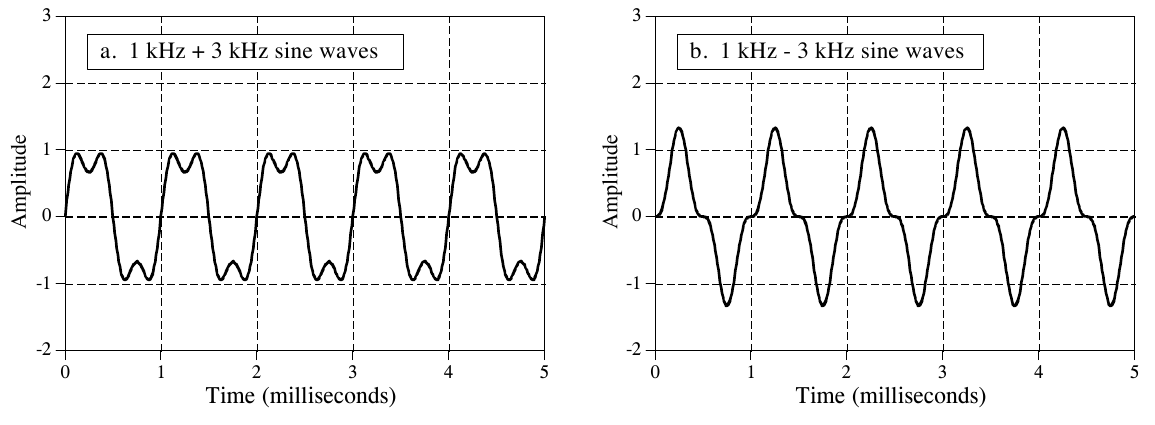
\includegraphics[width=0.963\linewidth,height=0.8\textheight,keepaspectratio]{assets/ch22/fig22-02.png}
\caption*{\textbf{图 22-2　人耳对相位的感知。}
人耳对各正弦分量之间的相对相位非常不敏感。例如，这两个波形听起来一模一样，因为它们各分量的幅度相同，尽管相对相位不同。
（a. 1 kHz + 3 kHz sine waves = 1 kHz 与 3 kHz 正弦波相加；b. 1 kHz − 3
kHz sine waves = 1 kHz 与 3 kHz 正弦波相减。Amplitude = 幅度，Time
(milliseconds) = 时间（毫秒）。）}
\end{figure}

考察声音在环境中怎样传播，就能理解耳朵为什么对相位不敏感。假设你在一个小房间里听对面的人说话。到达你耳朵的声音，很大一部分是从墙壁、天花板和地板反射来的。由于声音的传播与频率有关（比如衰减、反射和共振），不同频率会经由不同的路径到达你的耳朵。这意味着你在房间里走动时，各频率的相对相位会发生变化。由于耳朵忽略这些相位变化，你在移动时会觉得说话声没有变。从物理的角度看，音频信号在复杂环境中传播时，其相位会变得随机。换句话说，耳朵对相位不敏感，是因为相位几乎不含有用的信息。

不过，也不能说耳朵对相位完全充耳不闻。这是因为相位的改变可能会重新安排音频信号的时间顺序。一个例子是啁啾系统(chirp
system，第 11
章)，它把一个冲激变成一个持续时间长得多的信号。这两个声音虽然只在相位上不同，耳朵却能区分它们，因为它们的持续时间不同。这在很大程度上只是个奇特现象，在正常的听音环境中不会发生。

假设我们请一位小提琴手拉一个音，比如中央 C 下面的
A。在示波器上显示这个波形，它看起来很像图 22-3a
中的锯齿波(sawtooth)。这是小提琴弓毛上涂的黏性松香造成的。弓在弦上拉过时，弦先粘在弓上、被拉过去，最后挣脱开来，波形就这样形成了。这个循环一再重复，就得到了锯齿波形。

\begin{figure}[htbp]
\centering
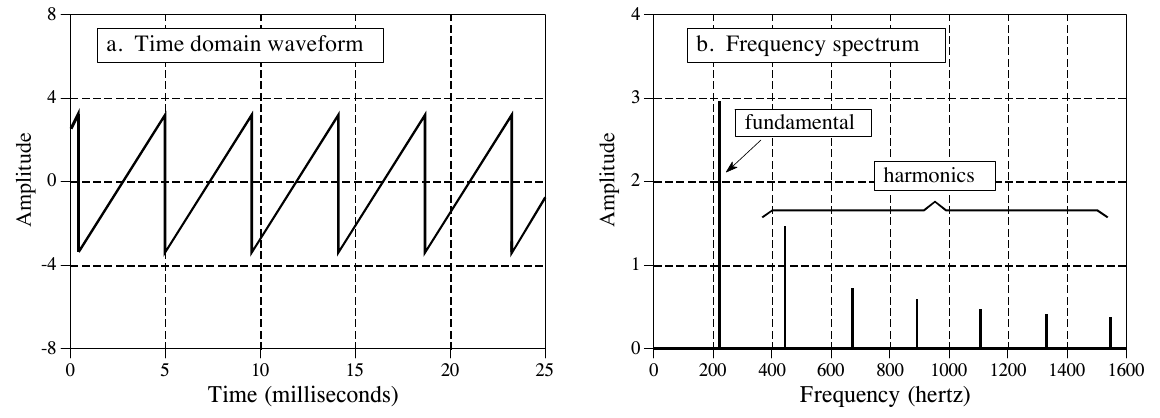
\includegraphics[width=0.967\linewidth,height=0.8\textheight,keepaspectratio]{assets/ch22/fig22-03.png}
\caption*{\textbf{图 22-3　小提琴的波形。} 拉奏的小提琴产生锯齿波，如 (a)
所示。耳朵听到的声音如 (b) 所示：基频加上各次谐波。 （a. Time domain
waveform = 时域波形；b. Frequency spectrum = 频谱，fundamental =
基频，harmonics = 谐波。Amplitude = 幅度，Time (milliseconds) =
时间（毫秒），Frequency (hertz) = 频率（赫兹）。）}
\end{figure}

图 22-3b 显示了耳朵怎样感知这个声音：220 Hz 的频率，加上 440、660、880
Hz
等处的谐波。如果在另一件乐器上奏出这个音，波形看起来会不同，但耳朵听到的仍然是
220 Hz
加上各次谐波。由于两件乐器奏这个音时产生相同的基频，它们听起来相似，称为音高相同。由于谐波的相对幅度不同，它们听起来又不会完全一样，称为音色不同。

人们常说音色由波形的形状决定。这话没错，但有点误导。音色的感知来自耳朵对谐波的检测。虽然谐波成分由波形的形状决定，但由于耳朵对相位不敏感，这种关系非常单向。也就是说，一个特定的波形只有一种音色，而一种特定的音色却对应无穷多种可能的波形。

耳朵非常习惯听''基频加谐波''。如果给听者放 1 kHz 和 3 kHz
两个正弦波的组合，他们会说听起来自然悦耳。如果换成 1 kHz 和 3.1 kHz
的正弦波，就会很难听。

这就是标准音阶的基础，如图 22-4
中的钢琴键盘所示。敲击钢琴最左边的键，产生 27.5 Hz 的基频，外加
55、110、220、440、880 Hz
等处的谐波（这些频率之间也有谐波，但对这里的讨论不重要）。这些谐波对应键盘上其他键产生的基频。具体来说，每隔七个白键，就是最左边那个键的一个谐波。也就是说，从左数第八个键的基频是
55 Hz，第 15 个键的基频是 110
Hz，依此类推。由于彼此互为谐波，这些键弹起来听着相似，一起弹时也很和谐。因此它们都叫做音符
A。同样，每个 A 右边紧挨着的白键叫
B，它们也都互为谐波。这个规律对七个音符 A、B、C、D、E、F、G 重复。

\begin{figure}[htbp]
\centering
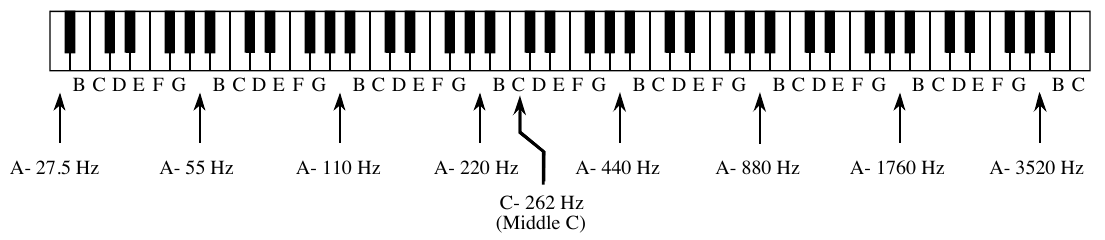
\includegraphics[width=0.921\linewidth,height=0.8\textheight,keepaspectratio]{assets/ch22/fig22-04.png}
\caption*{\textbf{图 22-4　钢琴键盘。}
钢琴键盘是一个对数频率刻度，每隔七个白键基频翻一倍。这些白键依次是音符
A、B、C、D、E、F 和 G。 （A- 27.5 Hz 等 = 各个 A 键的基频；C- 262 Hz
(Middle C) = 中央 C，262 Hz。）}
\end{figure}

八度(octave)这个术语指频率相差两倍。在钢琴上，一个八度包含八个白键，这就是名字的由来（octo
在拉丁语中是''八''）。换句话说，钢琴每隔七个白键频率翻一倍，整个键盘跨越七个多八度。人的听觉范围一般说是
20 Hz 到 20
kHz，大约相当于钢琴键盘左边再延伸半个八度、右边再延伸两个八度。由于八度是按每隔固定键数频率翻倍来定的，它是频率的一种对数表示。这一点很重要，因为音频信息一般也是这样分布的。例如，50
Hz 到 100 Hz 这一个八度所携带的音频信息，与 10 kHz 到 20 kHz
这一个八度一样多。尽管钢琴只覆盖人能听到的频率的约 20\%（20 kHz 中的 4
kHz），它却能产生人能感知的音频信息的 70\% 以上（10 个八度中的 7
个）。同样，在成年人的一生中，能听到的最高频率会从约 20 kHz 降到 10
kHz。但这只损失了约 10\%
的听力（十个八度中的一个）。下面会看到，信息的这种对数分布直接影响音频信号所需的采样率。

\section{音质与数据率}

设计数字音频系统时，要问两个问题：(1) 它需要听起来多好？(2)
能容忍多高的数据率？对这两个问题的回答通常落入三类中的一类。第一，高保真音乐，音质最重要，几乎任何数据率都能接受。第二，电话通信，要求语音听起来自然，同时数据率要低以降低系统成本。第三，压缩语音，降低数据率非常重要，音质上的一些不自然可以容忍。这包括军用通信、手机，以及用于语音信箱和多媒体的数字存储语音。

表 22-2
给出了这三类的音质与数据率之间的权衡。高保真音乐系统采样得足够快（44.1
kHz）、精度足够高（16
位），几乎能捕捉人能听到的所有声音。这种极好的音质是以高数据率为代价的：44.1
kHz × 16 位 = 706k 位/秒。这纯粹是蛮力。

音乐需要 20 kHz 的带宽，而听起来自然的语音只需要约 3.2
kHz。尽管频率范围降到了只有 16\%（20 kHz 中的 3.2
kHz），信号仍包含原来声音信息的 80\%（10 个八度中的 8
个）。电信系统通常以约 8 kHz
的采样率工作，语音听起来自然，但音乐质量大打折扣。你大概已经熟悉这种音质差别：FM
电台以将近 20 kHz 的带宽广播，而 AM 电台限制在约 3.2 kHz。在 AM
电台上人声听起来正常，音乐却单薄乏味。

只传语音的系统还把每个采样的精度从 16 位降到 12
位，音质几乎没有可察觉的变化。如果把量化步长做成不均匀的，还能降到每个采样只用
8 位。这是一种广泛使用的方法，叫压扩(companding)，本章后面会讲。8 kHz
的采样率配上每采样 8 位的 ADC 精度，得到 64k
位/秒的数据率。这是自然语音的''蛮力''数据率。注意语音所需的数据率还不到高保真音乐的
10\%。

\textbf{表 22-2　音频数据率与音质。}
数字化音频信号的音质取决于它的数据率，即采样率与每采样位数的乘积。可以分为三类：高保真音乐（706
k 位/秒）、电话质量语音（64 k 位/秒）和压缩语音（4 k 位/秒）。

\begingroup\footnotesize\setlength{\tabcolsep}{3pt}

{\def\LTcaptype{none} % do not increment counter
\begin{longtable}[]{@{}
  >{\raggedright\arraybackslash}p{(\linewidth - 10\tabcolsep) * \real{0.1667}}
  >{\raggedright\arraybackslash}p{(\linewidth - 10\tabcolsep) * \real{0.1667}}
  >{\raggedright\arraybackslash}p{(\linewidth - 10\tabcolsep) * \real{0.1667}}
  >{\raggedright\arraybackslash}p{(\linewidth - 10\tabcolsep) * \real{0.1667}}
  >{\raggedright\arraybackslash}p{(\linewidth - 10\tabcolsep) * \real{0.1667}}
  >{\raggedright\arraybackslash}p{(\linewidth - 10\tabcolsep) * \real{0.1667}}@{}}
\toprule\noalign{}
\begin{minipage}[b]{\linewidth}\raggedright
所需音质
\end{minipage} & \begin{minipage}[b]{\linewidth}\raggedright
带宽
\end{minipage} & \begin{minipage}[b]{\linewidth}\raggedright
采样率
\end{minipage} & \begin{minipage}[b]{\linewidth}\raggedright
位数
\end{minipage} & \begin{minipage}[b]{\linewidth}\raggedright
数据率（位/秒）
\end{minipage} & \begin{minipage}[b]{\linewidth}\raggedright
说明
\end{minipage} \\
\midrule\noalign{}
\endhead
\bottomrule\noalign{}
\endlastfoot
高保真音乐（CD） & 5 Hz～20 kHz & 44.1 kHz & 16 位 & 706k &
连最挑剔的发烧友也满意。比人的听觉还好。 \\
电话质量语音 & 200 Hz～3.2 kHz & 8 kHz & 12 位 & 96k &
语音质量好，但放音乐很差。 \\
（采用压扩） & 200 Hz～3.2 kHz & 8 kHz & 8 位 & 64k & 非线性 ADC
把数据率降低 50\%。非常常用的技术。 \\
线性预测编码的语音 & 200 Hz～3.2 kHz & 8 kHz & 12 位 & 4k & DSP
语音压缩技术。数据率很低，语音质量差。 \\
\end{longtable}
}

\endgroup

64k
位/秒的数据率代表把采样和量化理论直接用于音频信号的结果。进一步降低数据率的技术，都基于去除语音信号中固有的冗余来压缩数据流。数据压缩是第
27 章的主题。压缩音频信号最有效的方法之一是线性预测编码(Linear
Predictive Coding，LPC)，它有好几种变体和分支。根据所需的语音质量，LPC
能把数据率降到只有 2～6k 位/秒。本章后面讲语音合成时还会回到 LPC。

\section{高保真音频}

发烧友(audiophile)追求极致的音质，其他一切因素都是次要的。如果要用一个词来形容这种心态，那就是：过度(overkill)。这些系统不只是匹配人耳的能力，而是要超越听觉的极限。只有这样才能确保重放的音乐完美无瑕。数字音频是随激光唱片(compact
laser disc，即 CD)来到世间的。这是一场音乐的革命：CD
系统的音质远远超过唱片、磁带等老系统。DSP 一直站在这项技术的最前沿。

图 22-5
画出了激光唱片的表面，就像用高倍显微镜看到的那样。主表面是光亮的（能反光），数字信息存储为一串用激光烧在表面上的暗色凹坑(pit)。信息排成一条单独的轨道，从外向内螺旋，和黑胶唱片一样。从螺旋的外圈向内圈读取信息时，CD
的转速从约 210 rpm 变到 480 rpm，使扫描线速度保持恒定的 1.2
米/秒。（相比之下，黑胶唱片以固定转速旋转，比如 33、45 或 78
rpm。）播放时，一个光学传感器检测表面是反光还是不反光，生成相应的二进制信息。

\begin{figure}[htbp]
\centering
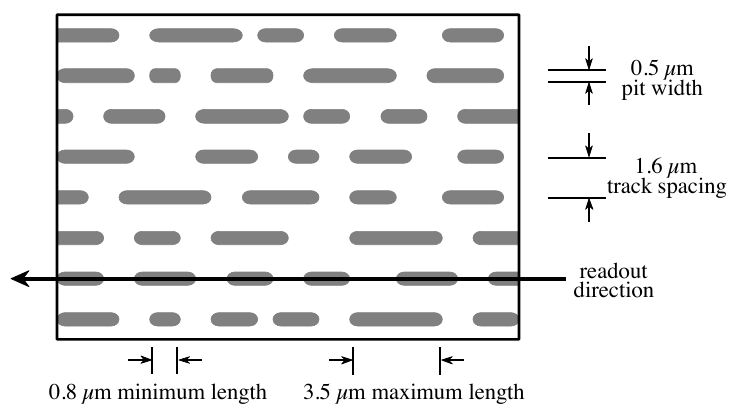
\includegraphics[width=0.617\linewidth,height=0.8\textheight,keepaspectratio]{assets/ch22/fig22-05.png}
\caption*{\textbf{图 22-5　CD 的表面。} 在 CD 表面烧出微米大小的凹坑来表示 1 和
0。由此得到的数据密度是每平方微米 1 位，即每平方毫米一百万位。凹坑深
0.16 µm。 （pit width = 凹坑宽度 0.5 µm，track spacing = 轨道间距 1.6
µm，readout direction = 读出方向，minimum length = 最短长度 0.8
µm，maximum length = 最长长度 3.5
µm。原书图注排在图左侧，裁图时已去掉，译文见上。）}
\end{figure}

按图 22-5 的几何尺寸，CD 每平方微米存储约 1
位，相当于每平方毫米一百万位，整张盘 150
亿位。这和集成电路制造所用的特征尺寸差不多，而且是有原因的。光的一个特性是：它不能被聚焦到小于约半个波长，即
0.3 µm。由于集成电路和激光唱片都是用光学手段制造的，光在 0.3 µm
以下的模糊限制了能用多小的特征尺寸。

图 22-6 是一个典型 CD 播放系统的框图。原始数据率是每秒 430
万位，相当于每 0.28 µm 轨道长度 1 位。然而，这与 CD
规定的几何尺寸冲突：每个凹坑不能短于 0.8 µm，也不能长于 3.5
µm。换句话说，每个二进制 1 都必须是一组 3 到 13 个 1
中的一部分。这样做的好处是降低光学读取头造成的误码率，但怎样迫使二进制数据服从这种奇怪的成组规则呢？

答案是一种叫八到十四调制(eight-to-fourteen
modulation，EFM)的编码方案。不是把一个字节的数据直接存到盘上，而是让这 8
位通过一张查找表，查出 14 位。这 14
位具备所需的成组特性，被存储到激光唱片上。播放时，从盘上读出的二进制值通过
EFM 查找表的逆表，每组 14 位又变回正确的 8 位。

\begin{figure}[htbp]
\centering
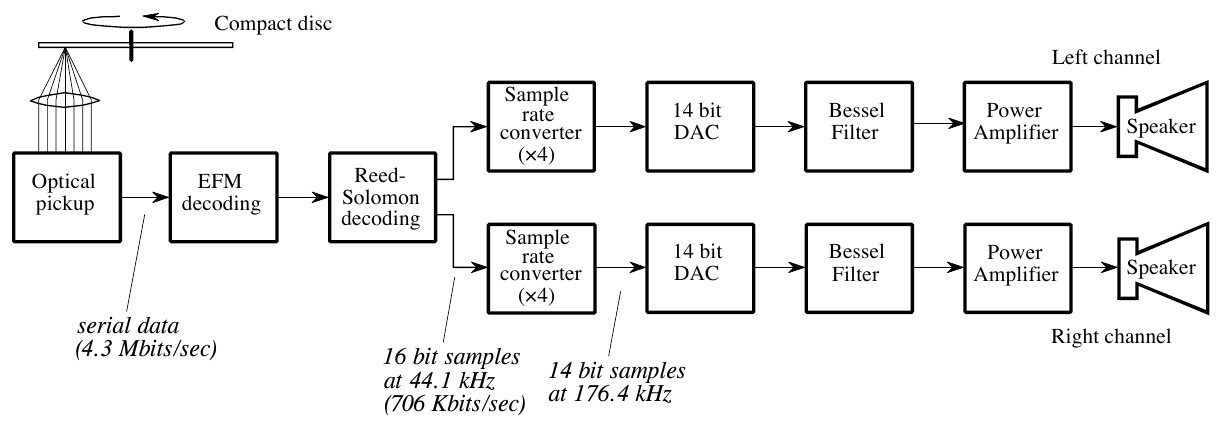
\includegraphics[width=1.000\linewidth,height=0.8\textheight,keepaspectratio]{assets/ch22/fig22-06.png}
\caption*{\textbf{图 22-6　CD 播放系统框图。} 用光学传感器从盘上取出数字信息，经过
EFM 解码和里德-所罗门(Reed-Solomon)解码校正，再转换成立体声模拟信号。
（Compact disc = 激光唱片，Optical pickup = 光学读取头，EFM decoding =
EFM 解码，Reed-Solomon decoding = 里德-所罗门解码，Sample rate converter
(×4) = 采样率转换器（×4），14 bit DAC = 14 位 DAC，Bessel Filter =
贝塞尔滤波器，Power Amplifier = 功率放大器，Speaker = 扬声器，Left /
Right channel = 左 / 右声道；serial data (4.3 Mbits/sec) = 串行数据（4.3
M 位/秒），16 bit samples at 44.1 kHz (706 Kbits/sec) = 44.1 kHz 的 16
位采样（706 k 位/秒），14 bit samples at 176.4 kHz = 176.4 kHz 的 14
位采样。）}
\end{figure}

除了 EFM，数据还以一种叫两级里德-所罗门编码(two-level Reed-Solomon
coding)的格式编码。这需要把左右两个立体声声道与用于检错和纠错的数据组合在一起。播放时检测到的数字错误，或者利用编码方案中的冗余数据纠正，或者通过在相邻采样之间插值来掩盖，或者把采样值设为零来静音。这些编码方案使数据率增加到三倍，即立体声音频信号的
1.4 M 位/秒对盘上存储的 4.3 M 位/秒。

解码和纠错之后，音频信号表示为 44.1 kHz 采样率下的 16
位采样。最简单的系统可以把这些信号送进一个 16 位
DAC，再接一个模拟低通滤波器。然而，这需要高性能的模拟电子电路，既要让 20
kHz 以下的频率通过，又要拒绝 22.05
kHz（采样率的一半）以上的所有频率。更常见的方法是使用多速率(multirate)技术，即在
DAC 之前把数字数据转换到更高的采样率。常用的倍数是四，从 44.1 kHz 转换到
176.4
kHz。这叫插值(interpolation)，可以解释为一个两步过程（尽管实际上未必这样实现）。第一步，在原来的采样之间插入三个值为零的采样，得到更高的采样率。在频域中，这相当于把
0～22.05 kHz 的频谱复制三次，分别位于 22.05～44.1 kHz、44.1～66.15 kHz
和 66.15～88.2
kHz。第二步，用一个高效的数字滤波器去掉新加进来的这些频率。

\begin{quote}
\textbf{译注：} 原书把第二段复制写成 ``41 to 66.15 kHz''，应为
44.1～66.15 kHz。
\end{quote}

提高采样率使采样间隔变小，DAC 生成的信号因此更平滑。信号仍然包含 20 Hz
到 20 kHz
之间的频率，但奈奎斯特频率提高到了四倍。这意味着模拟滤波器只需让 20 kHz
以下的频率通过，同时阻挡 88.2 kHz
以上的频率。这通常用一个三极点贝塞尔滤波器(Bessel
filter)来完成。既然耳朵对相位不敏感，为什么还要用贝塞尔滤波器？过度，记得吗？

由于采样多了三倍，每个采样的位数可以从 16 位降到 14
位，而音质不会下降。补偿 DAC 零阶保持(zeroth order hold)所需的 sin(x)/x
校正，可以放在模拟滤波器或数字滤波器中完成。

有多个声道的音频系统称为立体声(stereo，来自希腊语的''立体''，即三维的)。多个声道从不同方向向听者送出声音，更准确地再现原来的音乐。用单声道(monaural)系统播放的音乐往往听起来做作、平淡。相比之下，好的立体声重放让听者觉得乐手就在几步之外。从
1960
年代起，高保真音乐使用两个声道（左和右），而电影使用四个声道（左、右、中置和环绕）。在早期的立体声录音中（比如披头士或''妈妈与爸爸''乐队），常常只能在其中一个声道里听到某位歌手。这很快发展成更讲究的混缩(mix-down)，把录音棚里许多话筒的声音混合进两个声道。混缩是一门艺术，目的是让听者有身临其境的感觉。

电影中使用的四声道声音叫杜比立体声(Dolby
Stereo)，家用版本叫杜比环绕定向逻辑(Dolby Surround Pro
Logic)。（``Dolby'' 和 ``Pro Logic''
是杜比实验室许可公司的商标。）这四个声道被编码进标准的左右声道，使普通的双声道立体声系统也能重放这些音乐。播放时用杜比解码器重建出四个声道。左右声道来自放在电影或电视屏幕两侧的扬声器，和普通双声道立体声系统类似。中置声道的扬声器通常放在屏幕正上方或正下方。它的作用是重放语音和其他与画面相关的声音，使它们牢牢地居中于屏幕，不论观众/听众坐在哪里。环绕扬声器放在听者的左右两侧，在大礼堂中可能多达二十只。环绕声道只含中频（比如
100 Hz 到 7 kHz），并延迟 15 到 30
毫秒。这个延迟让听者觉得语音来自屏幕，而不是两侧。也就是说，听者先听到来自前方的语音，接着听到来自两侧的语音的延迟版本。听者的大脑把延迟的信号解释为墙壁的反射，从而忽略它。

\section{压扩}

数据率在电信中很重要，因为它与传输信号的成本成正比。省下比特就是省钱。压扩是降低音频信号数据率的一种常用技术，做法是让量化电平不均匀。前面说过，人能忍受的最响的声音（120
dB SPL）大约是能察觉的最弱声音（0 dB
SPL）幅度的一百万倍。然而，耳朵分辨不出相差小于约 1 dB（幅度
12\%）的声音。换句话说，在一百万倍的幅度范围内，能察觉的响度等级只有大约
120 个，而且按对数间隔分布。

这对音频信号的数字化很重要。如果量化电平等间距分布，要得到电话质量的语音必须用
12 位。然而，如果让量化电平不等间距、与人的听觉特性相匹配，只需要 8
位。这很直观：信号小的时候，电平要排得很密；信号大的时候，间距可以大一些。

压扩有三种实现方法：(1) 模拟信号先通过一个非线性电路，再进入线性的 8 位
ADC；(2) 使用内部台阶不等间距的 8 位 ADC；(3) 使用线性的 12 位
ADC，后面接一张数字查找表（输入 12 位，输出 8
位）。这三种方案需要的是同一个非线性，只是放在不同的地方：模拟电路、ADC
或数字电路。

压扩曲线有两个几乎相同的标准：北美使用的 µ255 律（µ255 law，也叫 µ 律(mu
law)），以及欧洲使用的 A 律(A
law)。两者都使用对数非线性，因为正是这种非线性把人耳能察觉的间距变换成线性间距。µ255
律和 A 律所用的曲线写成公式如下：

\textbf{公式 22-1}　µ 律压扩。这个公式给出 µ255 律压扩的非线性。常数 µ
的值为 255，标准由此得名。

\[y = \frac{\ln(1 + \mu x)}{\ln(1 + \mu)} \qquad 0 \le x \le 1\]

\textbf{公式 22-2}　A 律压扩。常数 A 的值为 87.6。

\[y = \begin{cases} \dfrac{1 + \ln(Ax)}{1 + \ln(A)} & 1/A \le x \le 1 \\[2ex] \dfrac{Ax}{1 + \ln(A)} & 0 \le x \le 1/A \end{cases}\]

图 22-7 画出了输入变量 x 在 −1 到 +1 之间时的这些曲线，输出变量也在 −1
到 +1 之间取值。公式 22-1 和 22-2
只处理正的输入值；负输入值部分的曲线由对称性得到。如 (a) 所示，µ255 律和
A 律的曲线几乎完全相同。唯一明显的差别在原点附近，如 (b) 所示：µ255
律是一条光滑曲线，而 A 律在这里换成了一条直线。

\begin{figure}[htbp]
\centering
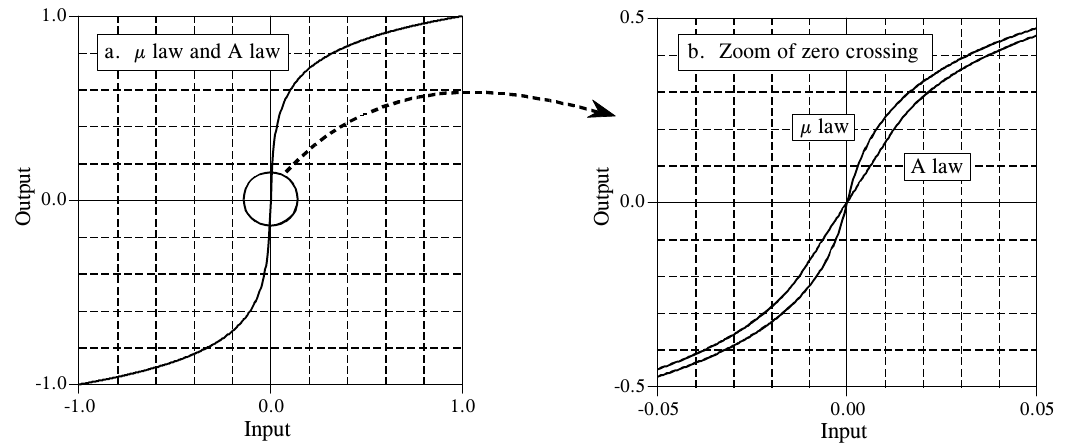
\includegraphics[width=0.892\linewidth,height=0.8\textheight,keepaspectratio]{assets/ch22/fig22-07.png}
\caption*{\textbf{图 22-7　压扩曲线。} µ255 律和 A
律的压扩曲线几乎完全相同，只在原点附近有差别。压扩在信号小的时候放大幅度，在信号大的时候减小幅度。
（a. µ law and A law = µ 律与 A 律；b. Zoom of zero crossing =
过零点附近放大。Input = 输入，Output = 输出。）}
\end{figure}

对模拟电子电路来说，做出一个稳定的非线性是件难事。一种方法是利用 PN
二极管结上电流与电压之间的对数关系，再加上电路来校正可怕的温度漂移。大多数压扩电路采用另一种策略：用一组直线段来近似这个非线性。一种典型方案是用
16 段直线来近似对数曲线，这些直线段叫弦(chord)。8
位输出的第一位表示输入是正还是负。接下来三位指出用的是 8 段正弦段或 8
段负弦段中的哪一段。最后四位把每段弦等分成 16
份。和大多数集成电路一样，压扩芯片的内部设计复杂且是专有的。与其操心芯片内部在干什么，不如把注意力放在引脚定义和规格书上。

\begin{quote}
\textbf{译注：} 原书把这些直线段拼成 cords（绳索），通行的术语是
chords（弦）。
\end{quote}

\section{语音合成与识别}

用计算机生成和识别语音是很难的问题；人们尝试了许多方法，成效都一般。这是
DSP
一个活跃的研究领域，无疑在今后许多年里也仍将如此。如果你指望这一节讲怎样搭建语音合成和识别电路，你会非常失望。这里只能简要介绍一下典型的方法。在开始之前应当指出，大多数能发出像人一样声音的商业产品并不是合成语音，而只是播放一段数字录制的真人语音。这种方法音质很好，但只限于预先录好的词语和短语。

几乎所有的语音合成与识别技术，都基于图 22-8
所示的人类发声模型。人的大多数语音可以分为浊音(voiced)和擦音(fricative)两类。浊音是空气从肺部被压出，经过声带(vocal
cords)，再从口和/或鼻出来时产生的。声带是喉结正后方横跨气流的两片薄薄的组织。随着肌肉张力的变化，声带以
50 到 1000 Hz
之间的频率振动，使一股股周期性的气流注入喉咙。元音就是浊音的例子。在图
22-8 中，浊音用脉冲串发生器表示，音高（即波形的基频）是一个可调参数。

\begin{figure}[htbp]
\centering
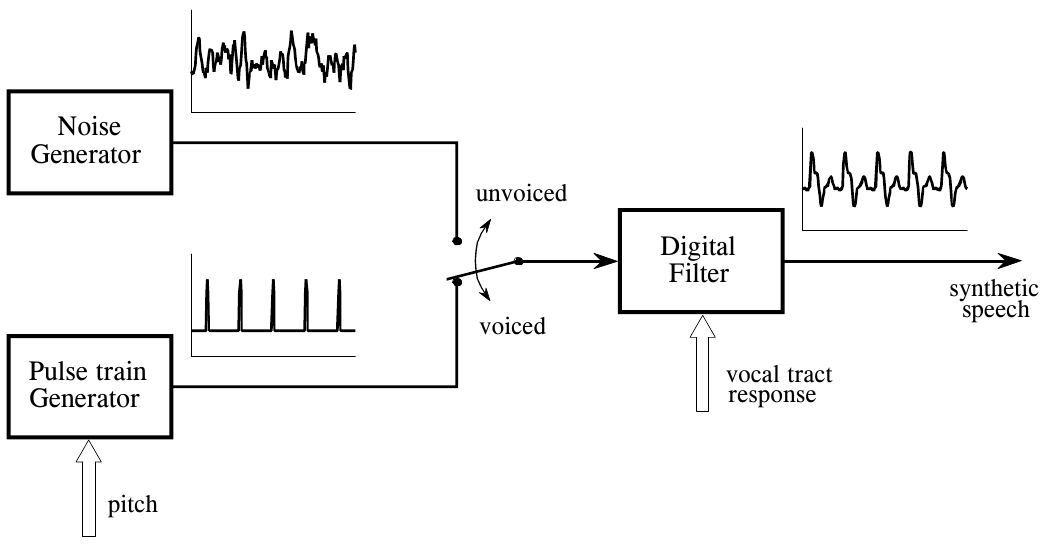
\includegraphics[width=0.867\linewidth,height=0.8\textheight,keepaspectratio]{assets/ch22/fig22-08.png}
\caption*{\textbf{图 22-8　人类发声模型。} 在一小段时间内（约 2 到 40
毫秒），语音可以用三个参数来建模：(1) 选择周期激励还是噪声激励；(2)
周期激励的音高；(3) 一个模仿声道响应的递归线性滤波器的系数。 （Noise
Generator = 噪声发生器，Pulse train Generator = 脉冲串发生器，pitch =
音高，unvoiced = 清音，voiced = 浊音，Digital Filter = 数字滤波器，vocal
tract response = 声道响应，synthetic speech = 合成语音。）}
\end{figure}

相比之下，擦音源于随机噪声，而不是声带的振动。当气流几乎被舌、唇和/或齿堵住，在收窄处附近产生湍流时，就会出现擦音。擦音包括
s、f、sh、z、v 和 th。在图 22-8 的模型中，擦音用噪声发生器表示。

这两种声源都要经过由舌、唇、口腔、咽喉和鼻腔形成的声学空腔的修饰。由于声音在这些结构中的传播是线性过程，可以用一个冲激响应选得合适的线性滤波器来表示。大多数情况下，模型中用的是递归滤波器，由递归系数决定滤波器的特性。由于这些声学空腔的尺寸有几厘米，频率响应主要是千赫兹范围内的一系列共振。在音频处理的行话里，这些共振峰叫共振峰频率(formant
frequencies)。改变舌和唇的相对位置，共振峰频率的频率和幅度都会随之改变。

\begin{quote}
\textbf{译注：} 原书把 formant frequencies 误拼成 format frequencies。
\end{quote}

图 22-9 是显示语音信号的一种常用方式：语谱图(voice
spectrogram)，也叫声纹(voiceprint)。把音频信号分成很短的段，比如 2 到 40
毫秒，用 FFT
求出每一段的频谱。把这些频谱并排放在一起，转换成灰度图像（幅度低的变浅，幅度高的变深）。这提供了一种图形化的方式，观察语音的频率成分怎样随时间变化。段的长度要在频率分辨率（段越长越好）和时间分辨率（段越短越好）之间折中。

\begin{figure}[htbp]
\centering
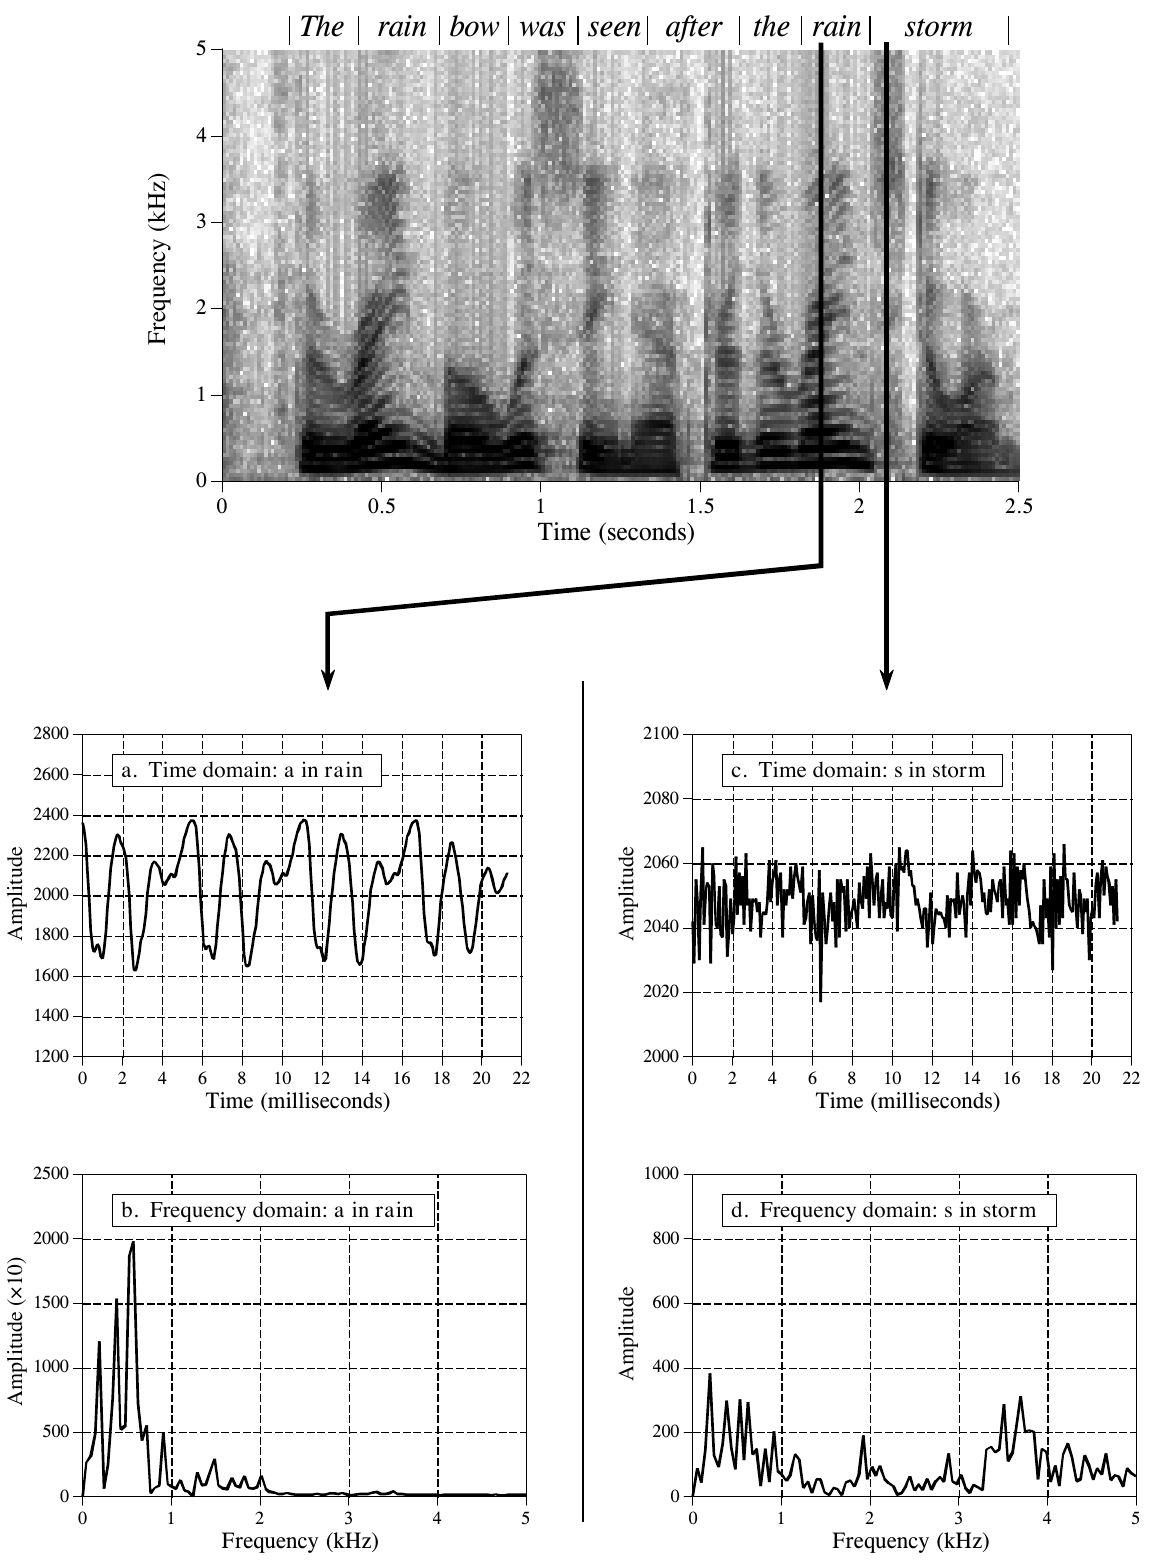
\includegraphics[width=0.958\linewidth,height=0.8\textheight,keepaspectratio]{assets/ch22/fig22-09.png}
\caption*{\textbf{图 22-9　语谱图。} 短语 ``The rainbow was seen after the rain
storm.''（雨后看到了彩虹）的语谱图。(a) 和 (b) 是 rain 中浊音 a
的时域和频域信号。(c) 和 (d) 是 storm 中擦音 s 的时域和频域信号。
（Frequency (kHz) = 频率（千赫），Time (seconds) = 时间（秒）；a. Time
domain: a in rain = 时域：rain 中的 a；b. Frequency domain: a in rain =
频域：rain 中的 a；c.~Time domain: s in storm = 时域：storm 中的
s；d.~Frequency domain: s in storm = 频域：storm 中的 s。Amplitude =
幅度，Amplitude (×10) = 幅度（×10），Time (milliseconds) =
时间（毫秒）。）}
\end{figure}

正如 rain 中的 a 所示，浊音的时域波形是周期的，如
(a)；频谱是一串等间距的谐波，如 (b)。相比之下，storm 中的 s
表明，擦音的时域信号是噪声状的，如 (c)；频谱也是噪声状的，如
(d)。这些频谱还显示出两种声音都受到共振峰频率的塑造。还要注意，rain
这个词说了两次，两次的时频图看起来很相似。

在一小段时间内（比如 25 毫秒），语音信号可以通过指定三个参数来近似：(1)
选择周期激励还是随机噪声激励；(2)
周期波的频率（如果用周期激励的话）；(3)
用来模仿声道响应的数字滤波器的系数。以每秒约 40
次的频率不断更新这三个参数，就能合成连续的语音。这种方法造就了 DSP
早期的商业成功之一：Speak \&
Spell（``说与拼''），一种广为销售的儿童电子学习机。这类语音合成的音质很差，听起来很机械，不太像人。不过它需要的数据率很低，通常只有几
k 位/秒。

这也是线性预测编码(LPC)语音压缩方法的基础。把数字录制的人类语音分成很短的段，每一段都按模型的三个参数来刻画。这通常每段需要大约一打字节，即每秒
2 到 6 k 字节。各段的信息按需要传输或存储，然后用语音合成器重建。

\begin{quote}
\textbf{译注：} 原书此处写 ``2 to 6 kbytes/sec''，与本章前文和表 22-2 的
2～6 k 位/秒不一致。按每段约 12 字节、每秒约 40 段计算，约为 0.5 k
字节/秒，即约 4 k 位/秒，应以''k 位/秒''为准。
\end{quote}

语音识别算法更进一步，试图在提取出的参数中识别模式。这通常需要把各段的信息与预先存储的声音模板进行比较，以求认出说的是哪些词。问题是，这种方法效果不太好。它对某些应用有用，但远远比不上人类听者的能力。要理解为什么语音识别对计算机来说这么难，设想有人突然说出下面这句话：

\begin{quote}
Larger run medical buy dogs fortunate almost when.（逐词直译：``更大 跑
医疗的 买 狗 幸运的 几乎 当\ldots\ldots 时''。）
\end{quote}

当然，你不会明白这句话的意思，因为它根本没有意思。更重要的是，你很可能连说出的每个词都听不全。这正是人类感知和理解语音方式的基本特点。词语是靠它们的声音识别的，但也靠句子的上下文和听者的预期。例如，设想听到下面两句话：

\begin{quote}
The child wore a spider ring on
Halloween.（孩子在万圣节戴了一枚蜘蛛戒指。）

He was an American spy during the war.（他在战争期间是一名美国间谍。）
\end{quote}

\begin{quote}
\textbf{译注：} 原书两句中加下划线的部分分别是 spider ring 和 spy
during，两者发音几乎相同。
\end{quote}

即使用来传达划线词语的声音完全相同，听者也会根据上下文听出正确的词。凭着你积累的关于世界的知识，你知道孩子不会''戴''特工，人也不会在战时变成吓人的首饰。这通常不是有意识的行为，而是人类听觉固有的一部分。

大多数语音识别算法只依赖单个词的声音，而不依赖上下文。它们试图识别词语，而不是理解语音。这使它们与人类听者相比处于极大的劣势。语音识别系统中常见三种令人烦恼的限制：(1)
被识别的语音必须在词与词之间有明显的停顿。这样算法就不必处理那些听起来相似、却由不同的词组成的短语（比如
spider ring 和 spy during）。对于习惯连贯说话的人来说，这既慢又别扭。(2)
词汇量往往只限于几百个词。这意味着算法只需在有限的集合中搜索最佳匹配。词汇量越大，识别时间和错误率都会增加。(3)
算法必须针对每个说话人进行训练。这需要每个使用系统的人把每个待识别的词说一遍，通常要重复五到十次。这种个性化的数据库大大提高了词语识别的准确率，但既不方便又费时间。

开发出成功的语音识别技术，回报是巨大的。语音是人类最快、最有效的交流方式。语音识别有可能取代书写、打字、键盘输入，以及由开关和旋钮提供的电子控制。它只需要再好用一点，就能被商业市场接受。语音识别的进步很可能既来自
DSP
本身，也同样来自人工智能和神经网络领域。别把这看作技术上的困难，把它看作技术上的机遇。

\section{非线性音频处理}

数字滤波能在许多方面改善音频信号。例如，维纳滤波(Wiener
filtering)可以把主要是信号的频率与主要是噪声的频率分开（见第 17
章）。同样，反卷积(deconvolution)可以补偿不想要的卷积，比如修复老录音（也在第
17 章讨论）。这类线性技术是 DSP
的支柱。还有几种非线性技术对音频处理也很有用。这里简要介绍其中两种。

第一种非线性技术用来降低语音信号中的宽带噪声。这类噪声包括：磁带嘶声、模拟电路中的电子噪声、风吹过话筒的声音、人群欢呼声等。线性滤波在这里没什么用，因为噪声的频率与语音信号的频率完全重叠，两者都覆盖
200 Hz 到 3.2 kHz
的范围。两个信号在时域和频域都重叠时，怎样才能把它们分开？

做法是这样的。在一小段语音中，各频率成分的幅度极不均匀。例如，图 22-10a
是一段 16 毫秒语音（即 8 kHz 采样率下的 128
个采样）的频谱。大部分信号集中在少数几个幅度大的频率上。相比之下，(b)
是只有随机噪声时的频谱；它非常不规则，但分布得更均匀，幅度也低。

\begin{figure}[htbp]
\centering
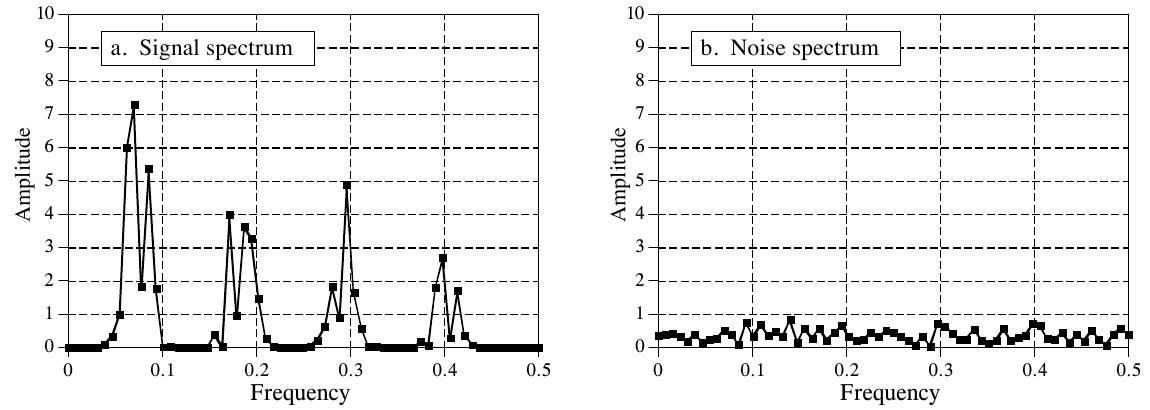
\includegraphics[width=0.958\linewidth,height=0.8\textheight,keepaspectratio]{assets/ch22/fig22-10.png}
\caption*{\textbf{图 22-10　语音和噪声的频谱。}
语音和噪声的频谱一般是重叠的，但如果信号段取得足够短，两者就会有一定程度的分离。(a)
是一段 16
毫秒语音的频谱，显示在这一特定段中，许多频率几乎不携带语音信息。(b)
是一个随机噪声源的频谱，所有分量的幅度都很小。（这些图不是真实信号，而是为了说明降噪技术画的示意图。）
（a. Signal spectrum = 信号频谱；b. Noise spectrum = 噪声频谱。Amplitude
= 幅度，Frequency = 频率。）}
\end{figure}

现在是关键的概念：如果信号和噪声同时存在，可以通过查看每个频率的幅度把两者部分地分开。如果幅度大，它很可能主要是信号，因此应当保留。如果幅度小，可以认为它主要是噪声，因此应当丢弃，即设为零。中等大小的频率分量在这两个极端之间以某种平滑的方式调整。

看待这种技术的另一种方式，是把它当作一个时变的维纳滤波器。你应该还记得，维纳滤波器的频率响应让主要是信号的频率通过，拒绝主要是噪声的频率。这需要预先知道信号和噪声的频谱，才能确定滤波器的频率响应。这种非线性技术用的是同样的思想，只是维纳滤波器的频率响应针对每一段、根据该段的频谱重新计算。换句话说，滤波器的频率响应逐段变化，由信号本身的特性决定。

实现这种（以及其他）非线性技术的困难之一，是用来对长信号滤波的重叠相加法(overlap-add
method)不再有效。由于频率响应在变化，各段的时域波形不再与相邻段对齐。要克服这一点，可以记住：音频信息编码在随时间变化的频率模式中，而不是在时域波形的形状中。一种典型做法是把原来的时域信号分成相互重叠的段。处理之后，在重新合并之前给每个重叠段加一个平滑的窗。这样频谱从一段到下一段就能平滑过渡。

第二种非线性技术叫同态信号处理(homomorphic signal
processing)。这个术语的字面意思是''相同的结构''。噪声和干扰与有用信号的结合方式不只有相加；相乘和卷积也是信号混合的常见方式。如果信号以非线性方式（即相加以外的任何方式）结合，就无法用线性滤波把它们分开。同态技术试图把问题变成线性的，从而分开以非线性方式结合的信号。也就是说，把问题转换成与线性系统相同的结构。

例如，考虑一个经由 AM
无线电波传输的音频信号。随着大气条件的变化，接收到的信号幅度时大时小，使接收到的音频信号的响度随时间缓慢变化。这可以建模为音频信号
a{[} {]} 乘以一个缓慢变化的信号 g{[}
{]}，后者代表不断变化的增益。这个问题通常用一种叫自动增益控制(automatic
gain control，AGC)的电子电路来处理，但也可以用非线性 DSP 来校正。

如图 22-11 所示，输入信号 a{[} {]}×g{[} {]} 通过对数函数。根据恒等式
\(\log(x \times y) = \log x + \log y\)，得到两个以相加方式结合的信号，即
log a{[} {]} + log g{[}
{]}。换句话说，对数就是把相乘这个非线性问题变成相加这个线性问题的同态变换。

\begin{quote}
\textbf{译注：} 原书这个恒等式印成了 log(x + y) = log x + log y，应为
log(x × y)。
\end{quote}

\begin{figure}[htbp]
\centering
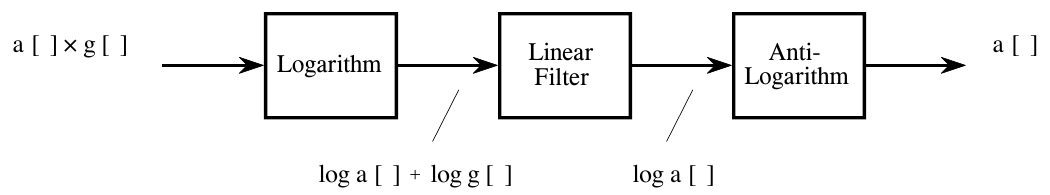
\includegraphics[width=0.875\linewidth,height=0.8\textheight,keepaspectratio]{assets/ch22/fig22-11.png}
\caption*{\textbf{图 22-11　相乘信号的同态分离。}
对输入信号取对数，把相乘的分量变成相加的分量。然后可以用线性滤波把这些分量分开，再撤销对数的作用。
（Logarithm = 对数，Linear Filter = 线性滤波器，Anti-Logarithm =
反对数。）}
\end{figure}

接下来，用常规的线性滤波器把相加的信号分开，也就是让一些频率通过、拒绝另一些频率。对于
AGC，增益信号 g{[} {]} 由非常低的频率组成，远低于语音信号 200 Hz 到 3.2
kHz
的频带。这些信号取对数后的频谱会更复杂，但思路是一样的：用一个高通滤波器把变化的增益分量从信号中去掉。

实际上，log a{[} {]} + log g{[} {]} 被变成了 log a{[}
{]}。最后一步，用指数函数（反对数，即
\(e^x\)）撤销对数，得到所需的输出信号 a{[} {]}。

图 22-12
是一个分离卷积信号的同态系统。这已被证明有用的一个应用是去除音频信号中的回声。也就是说，音频信号与一个由''冲激函数加上一个平移并缩放过的冲激函数''构成的冲激响应卷积在了一起。卷积的同态变换由两级组成：先做傅里叶变换，把卷积变成相乘；再取对数，把相乘变成相加。和前面一样，接着用线性滤波把信号分开，再撤销同态变换。

\begin{figure}[htbp]
\centering
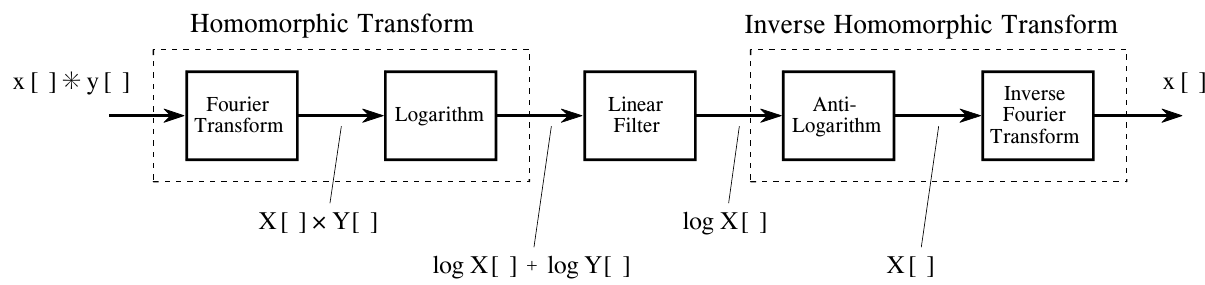
\includegraphics[width=1.000\linewidth,height=0.8\textheight,keepaspectratio]{assets/ch22/fig22-12.png}
\caption*{\textbf{图 22-12　卷积信号的同态分离。}
先做傅里叶变换再取对数，把卷积在一起的分量变成相加的分量。用线性滤波分开这些相加的分量之后，再按原来的步骤逐一撤销。
（Homomorphic Transform = 同态变换，Inverse Homomorphic Transform =
逆同态变换，Fourier Transform = 傅里叶变换，Logarithm = 对数，Linear
Filter = 线性滤波器，Anti-Logarithm = 反对数，Inverse Fourier Transform
= 逆傅里叶变换；x{[} {]} \dspsym{∗} y{[} {]} 中的 \dspsym{∗} 是卷积。）}
\end{figure}

图 22-12
有一个有趣的转折：线性滤波处理频域信号的方式，和通常处理时域信号的方式一样。换句话说，时域和频域的角色与平常互换了。例如，如果用
FFT
卷积来完成线性滤波这一级，被相乘的''频谱''就会位于时域。这种角色反转催生了一套奇怪的行话。例如，倒谱(cepstrum，把
spectrum
的字母重新排列而成)是傅里叶变换的对数的傅里叶变换。同样，有长通(long-pass)和短通(short-pass)滤波器，而不是低通和高通滤波器。有些作者甚至使用''倒频分析''(Quefrency
Alanysis，由 Frequency Analysis 换字母而来)和''倒滤波''(liftering，由
filtering 换字母而来)这样的说法。

请记住，这些只是对复杂 DSP
算法的简化描述；同态处理充满了微妙的细节。例如，对数必须能处理输入信号中的负值和正值，因为音频信号就有这个特点。这需要用到复对数(complex
logarithm)，它比日常科学和工程中用的对数更高深。如果把线性滤波限制为零相位滤波器，复对数可以通过对信号的绝对值取普通对数求得。通过零相位滤波器之后，再把原信号的符号重新加到滤波后的信号上。

另一个问题是取对数时出现的混叠。例如，设想对一个连续正弦波做数字化。根据采样定理，每个周期两个或更多采样就够了。现在考虑对这个连续正弦波的对数做数字化。它的尖角需要每个周期多得多的采样才能把波形捕捉下来，也就是防止混叠。取对数之后所需的采样率很容易达到之前的
100
倍。而且，对数是作用在连续信号上还是它的数字表示上，结果都一样。除非采样率高到能捕捉非线性产生的尖角，否则就会发生混叠。结果是音频信号可能需要以
100 kHz 或更高的频率采样，而不是标准的 8 kHz。

即使处理好了这些细节，也不能保证线性化后的信号可以被线性滤波器分开。这是因为即使原信号的频谱不重叠，线性化后信号的频谱也可能重叠。例如，设想把两个正弦波相加，一个
1 kHz，一个 2
kHz。由于这两个信号在频域中不重叠，可以用线性滤波把它们完全分开。现在设想把这两个正弦波相乘。用同态处理，对组合后的信号取对数，得到一个正弦波的对数加上另一个正弦波的对数。问题是，正弦波的对数含有许多谐波。由于两个信号的谐波相互重叠，不可能把它们完全分开。

尽管有这些障碍，同态处理教给我们一个重要的道理：处理信号的方式应当与信号形成的方式相一致。换句话说，任何
DSP 任务的第一步，都是弄清信息在所处理的信号中是怎样表示的。
